\chapter{Il livello di link e LANs}
Esistono due tipi di canali a livello di link: il primo tipo sono i canali broadcast che connettono multipli host e rendono necessario un access medium protocol; il secondo tipo \`e il link di comunicazione punto a 
punto.
\section{Introduzione}
Si indica un oggetto che esegue un protocollo di livello di link come ad un nodo che includono host, router, switches e WIFI access point. Ci si riferisce ai canali di comunicazione che connettono i nodi adiacenti 
come links. In modo che un datagramma sia trasferito da un host source a uno di destinazione si deve muovere lungo ognuno dei link individuali nel cammino. Su un dato link un modo trasmettitore incapsula
il datagramma in un frame di livello di link e lo trasmette nel link. 
\subsection{Servizi messi a disposizione}
Nonostante il servizio base di ogni livello di link \`e di spostare un datagramma da un nodo all'adiacente lungo un singolo link di comunicazione ci sono altre funzionalit\`a che dipendono dal protocollo:
\begin{itemize}
\item Framing: quasi tutti i protocolli di livello di link incapsulano ogni datagramma di livello di rete in un frame prima di trasmetterlo lungo il link. Un frame consiste in un campo di dati dove si trova il payload e 
un numero di campi di header. 
\item Link access: un protocollo di medium access control (MAC) specifica le regole secondo cui un frame \`e trasmesso lungo il link. Il protocollo diventa naturalmente pi\`u complesso per i canali broadcast in 
quanto coordina la trasmissione dei frame ai vari nodi.
\item Reliable deliver: quando il protocollo la mette a disposizione garantisce di muovere ogni datagramma lungo il link senza errori.  Similarmente  a TCP pu\`o essere ottenuto con ACK e ritrasmissioni. Questo
si fa nel tentativo di correggere l'errore localmente. Maggiormente diffuso per i link wireless.
\item Error detection and correction: l'hardware del livello di link in un nodo ricevente potrebbe flippare erroneamente un bit. In quanto sarebbe inutile continuare l'invio del pacchetto molti protocolli mettono
a disposizioni metodi per individuare tali errori. \`E ottenuto attraverso l'aggiunta di bit per questo scopo attraverso tecniche pi\`u sofisticate dei livelli superiori e implementazione hardware. Per la correzione di
tali errori si rende necessario capire in quali bit \`e avvenuto l'errore.  
\end{itemize}
\subsection{Implementazione del livello di link}
Nei router \`e implementato nelle line cards. Per la maggior parte il livello di link \`e implementato in un network adapter (network interface card o NIC), nel cui cuore si trova il controller del livello di link, un chip
special purpose che implementa molti dei servizi. Dal lato mittente il controller prende un datagramma che \`e stato creato e salvato nella memoria dell'host dai livelli superiori, lo incapsula in un frame 
riempiendo i campi dell'header e lo trasmette nel link di comunicazione attraverso il protocollo di link-access. Dal lato del ricevente un controller riceve un frame ed estrae il datagramma del livello di rete. Se 
esegue error detection il mittente setta i bits necessari nell'header e il ricevente esegue l'error detection. Le parti implementate in software mettono a disposizioni funzionalit\`a di alto livello come assemblare
indirizzamento di livello di link e attivare il controller hardware. Dal lato del ricevente il software risponde ad un controller interrupt gestisce le condizioni di errore i passa il datagramma ai livelli successivi. 
\section{Tecniche di individuazione e correzione errori}
Al nodo inviante i dati D che devono essere protetti da errori sono aumentati con bit di individuazione e correzione errori (EDC), tali dati sono composti dal datagramma, informazioni di indirizzamento di livello 
di link, numeri di sequenza e altri campi nel frame header. Sia D che EDC sono inviati al nodo ricevente in un frame. Al nodo ricevente una sequenza di bit D' e EDC' sono ricevuti. A causa di errori i primi e i 
secondi potrebbero variare. Il ricevente deve essere in grado di determinare se sono diversi. Queste tecniche non sono perfette. Tecniche pi\`u sofisticate richiedono overhead maggiori.
\subsection{Parity checks}
Questo metodo di individuazione errori consiste nell'utilizzo di un singolo parity bit. Si supponga che l'informazione da inviare D ha $d$ bit. In un even parity scheme il mittente include un bit aggiuntivo e 
sceglie il suo valore tale che il numero totale di uni nei bit $d+1$ \`e pari. Il ricevente deve solo contare i numeri di uni nei $d+1$ bit. Se \`e dispari c'\`e un errore, altrimenti no. Se succede un numero pari di bit 
errors l'errore non viene individuato. Si pu\`o fare una generalizzazione bidimensionale in cui i $d$ bit sono divisi in $i$ righe e $j$ colonne. Un valore di parity \`e computato per ogni riga e per ogni colonna. I 
risultanti $i+j+1$ parity bit sono inclusi nel campo appropriato. Con questo schema bidimensionale quando accade un errore la parity sia della colonna che della riga sono sbagliate e pertanto si pu\`o 
identificare il bit singolo sbagliato e correggerlo (se c'\`e un singolo errore). L'abilit\`a per un ricevente di individuare e correggere errori \`e conosciuta come forward error correction (FEC). 
\subsection{Checksumming methods}
Questo metodo di individuazione consiste nel trattare i $d$ bit di dati come una sequenza di $k$-bit integer. Un semplice metodo consiste nel sommare questi interi e utilizzare tale somma come i bit per l'error
detection. L'internet checksum \`e basato su questo approccio. 
\subsection{Cyclic redundancy check (CRC)}
Questa tecnica utilizzata in larga scala \`e basata sui codici di cyclic redundancy check. Sono conosciuti come codici polinomiali in quanto \`e possibile considerare la stringa di bit come un polinomio i cui 
coefficienti sono i valori 0 e 1 con operazioni sulla stringa di bit interpretate come aritmetica polinomiale. Si consideri il dato D di $d$ bit che il mittente vuole inviare. Il mittente e il ricevente devono prima 
mettersi d'accordo su un pattern a $r+1$ bit conosciuto come un generatore che si denota con G. Si impone che il bit pi\`u significativo di G sia 1. Per un dato il mittente sceglie $r$ bit addizionali $R$ e li 
aggiunge a D in modo che il pattern $d+r$ interpretato come un numero binario sia esattamente divisibile da G utilizzando l'aritmetica modulo 2. Il processo di controllo errori consiste nella divisione da parte 
del ricevente dei $d+r$ bit ricevuti con G. Se il rimanente \`e non zero il ricevente sa che c'\`e stato un errore, altrimenti i dati sono accettati come corretti. Utilizzando l'aritmetica modulo due senza riporti
sottrazione e addizione si computano attraverso XOR, mentre moltiplicazione e divisione attraverso shift. Pertanto dati D e R la quantit\`a $D\cdot 2r XOR R$ contiene i $d+R$ bit. Si deve pertanto capire come
il mittente computa $R$. Considerando l'equazione precedente si pu\`o calcolare $R=D2r\mod G$. Gli standard CRC possono individuare burst errors di meno di $r+1$ bit. Sotto certe assunzioni possono 
individuare i burst error maggiori con probabilit\`a $1-0.5r$, possono individuare ogni numero dispari di errori. 
\section{Access links multipli e protocolli}
Un link point-to-point consiste di un singolo mittente a un capo e in singolo ricevente all'altro. Molti protocolli di livello di link sono stati costruiti per questo scopo. Un altro tipo di link \`e un link broadcast che 
pu\`o avere multipli mittenti e riceventi tutti connessi allo stesso condiviso canale broadcast. Quando un nodo trasmette un frame tutti i nodi connessi al link ne ricevono una copia. Ne sono un esempio 
ethernet e wireless LAN. Si vedr\`a come gestire il problema del multiplo accesso. Vengono pertanto creati protocolli di accesso multiplo secondo i quali i nodi regolano la loro trasmissione sul canale condiviso.
Essendo che tutti i nodi sono capaci di trasmettere frame possono inviarli allo stesso momento e i frame collidono a tutti i riceventi. Quando c'\`e una collisione i segnali dei frames si ingarbugliano tra di loro. 
Diventa pertanto necessario coordinare la trasmissione dei nodi attivi, lavoro svolto dal protocollo di accesso multiplo. Questi protocolli si possono dividere in channel partitioning, random access e taking-
turns. Questi protocolli per un canale con tasso di trasmissione di $R\frac{bits}{second}$ dovrebbero:
\begin{itemize}
\item Quando solo un nodo deve trasmettere dei dati il suo throughput deve essere $R$.
\item Quando $M$ nodi devono trasmettere ognuno di essi deve avere un throughput di $\frac{R}{M}$ come tasso di trasmissione medio.
\item Il protocollo \`e decentralizzato.
\item Il protocollo \`e semplice e poco costoso da implementare.
\end{itemize}
\subsection{Protocolli di channel partitioning}
Time division-multiplexing (TDM) e frequency-division multiplexing (FDM) sono due tecniche utilizzate per partizionare la bandwidth di un canale broadcast tra tutti i nodi che condividono il canale. TDM divide
il tempo in time frames e divide ogni time frame in time slots pari al numero di nodi nel canale. Ogni time slot \`e assegnato ad uno dei nodi. Ogniqualvolta un nodo deve trasmettere un pacchetto lo trasmette
durante il suo assegnato time slot nel corrente TDM frame. Le dimensioni degli slot sono decise in modo che un singolo pacchetto possa essere trasmesso durante uno slot time.   FDM divide il canale in 
frequenze diverse invece di time slots e assegna una frequenza ad ogni nodo. Entrambi eliminano le collisioni e sono perfettamente fair, ma un nodo deve aspettare sempre il suo momento anche se \`e l'unico 
che deve inviare un pacchetto. Un terzo protocollo di questo tipo \`e il code division multiple access (CDMA) che assegna un codice diverso ad ogni nodo che lo utilizza per codificare i dati che invia. Se i codici
sono scelti accuratamente i nodi diversi possono trasmettere simultaneamente e avere i destinatari ricevere correttamente i dati codificati se conosce il codice del mittente. 
\subsection{Random access protocols}
In questi protocolli un nodo trasmette al tasso pieno. Quando c'\`e una collisione tutti i nodi coinvolti aspettano un tempo randomico prima di ritrasmettere il pacchetto. 
\subsubsection{Slotted ALOHA}
Si assuma che tutti i frame consistano di $L$ bit, il tempo \`e diviso in slot di dimensione $\frac{L}{R}$, i nodi cominciano a trasmettere frames solo all'inizio degli slot, sono sincronizzati in modo che ogni nodo
sa quando lo slot comincia, se due o pi\`u frame collidono in uno slot tutti i nodi individuano la collisione prima che lo slot finisce. Sia $p$ una probabilit\`a, le operazioni dello slotted ALOHA in ogni nodo sono:
\begin{itemize}
\item Quando un nodo ha un nuovo frame da inviare aspetta fino all'inizio del prossimo e trasmette l'intero frame nello slot.
\item Se non c'\`e collisione il nodo \`e stato trasmesso con successo.
\item Se c'\`e collisione il nodo la individua prima della fine dello slot e ritrasmette il frame in ogni slot seguente con probabilit\`a $p$ fino a che il frame \`e trasmesso senza collisione. La propriet\`a di un nodo
\`e indipendente da quella negli altri.
\end{itemize}
A differenza del channel partitioning permette ad un nodo di trasmettere continuamente al tasso pieno ed \`e altamente decentralizzato, anche se richiede una sincronizzazione degli slot. Quando c'\`e una 
collisione \`e possibile perdere uno slot, alcuni slot possono rimanere vuoti. Uno slot non sprecato si dice successful. L'efficienza di uno slotted multiple accesso protocol \`e definita come la frazione di slots
successful nella long-run, Supponendo che ogni nodo provi a trasmettere un frame in ogni slot con probabilit\`a $p$ e che ci siano $N$ nodi.  La probabilit\`a che un dato slot sia successful \`e la probabilit\`a che
un nodo trasmetta: $p\frac{1-p}{N-1}$. La probabilit\`a che un nodo abbia un successo \`e $Np\frac{1-p}{N-1}$ che \`e l'efficienza del protocollo slotted ALOHA. Per ottimizzare l'efficienza si deve trovare la
probabilit\`a $p*$ per cui quel valore \`e massimo e per un grande numero di nodi si prende il limite a infinito di $Np*\frac{1-p*}{N-1}$. La massima efficienza \`e  $\frac{1}{e}$, ovvero al meglio solo il $37\%$ 
degli slot fa del lavoro utile, lo stesso numero di slot rimangono vuoti e nel $26\%$ ci sono collisioni. 
\subsubsection{ALOHA}
In ALOHA puro non esistono gli slot: quando arriva un frame il mittente lo trasmette immediatamente. Se c'\`e una collisione il nodo lo ritrasmette immediatamente con probabilit\`a $p$ o aspetta per un 
frame transmission time e ripete. Per determinare la massima efficienza ci si concentri su un nodo individuale e il frame transmission time un unit\`a di tempo. Ad ogni momento la probabilit\`a che un nodo 
stia trasmettendo un frame \`e $p$. Si supponga che inizi la trasmissione a tempo $t_0$, pertanto nessun altro nodo pu\`o iniziare a  trasmettere nell'intervallo $[t_0-1, t_0]$ in quanto le trasmissioni si 
sovrapporrebbero. La probabilit\`a di una trasmissione con successo \`e $p\frac{1-p}{2(N-1)}$. Si trova che la massima efficienza \`e $\frac{1}{2e}$, la met\`a dello slotted ALOHA, il prezzo per un protocollo
completamente decentralizzato. 
\subsubsection{Carrier Sense Multiple Access (CSMA)}
Si dice carrier sensing il fatto che un nodo ascolta il canale prima di trasmettere. Se un frame sta venendo trasmesso aspetta fino a che non individua nessuna trasmissione per un breve periodo prima di 
cominciare la trasmissione. Si dice collision detection il fatto che un nodo trasmettente ascolta il canale mentre trasmette e se individua che un altro nodo sta trasmettendo blocca la sua trasmissione e aspetta
un randomico tempo prima di ripetere il processo di sense-and-transmit-when-idle. Queste regole sono caratteristiche della famiglia dei carrier sense multiple access (CSMA) e CSMA con collision detection
(CSMA/CD). Questi protocolli non evitano completamente collisioni a causa del channel propagation delay. La probabilit\`a di collisioni \`e direttamente proporzionale a questo ritardo.
\subsubsection{Carrier sense multiple access con collision detection (CSMA/CD)}
Quando un nodo svolge la collision detection smette la trasmissione appena individua una collisione. Aumenta le prestazioni in quanto riduce i frame inutili trasmessi. Le operazioni di questo protocollo sono:
\begin{itemize}
\item L'adattatore riceve un datagramma dal livello di rete, prepara il frame e lo mette nel buffer.
\item Se l'adattatore percepisce che il canale \`e in quiete comincia la trasmissione del frame. Se percepisce che \`e occupato aspetta fino a che entra in quiete.
\item Mentre trasmette l'adattatore monitora per la presenza di segnali che arrivano da altri adattatori nel canale.
\item Se l'adattatore trasmette l'intero frame senza percepire nessun'altra trasmissione termina il frame, altrimenti fa abort della trasmissione.
\item Dopo l'abort l'adattatore aspetta un tempo randomico e ritorna al secondo passo.
\end{itemize}
La necessit\`a di aspettare un tempo randomico \`e per impedire collisioni infinite. La dimensione dell'intervallo \`e determinata dall'algoritmo di binary exponential backoff. Quando si trasmette un frame che ha
gi\`a avuto $n$ collisioni un nodo sceglie un valore di $K$ a caso tra $[0,2n-1]$, che pertanto aumenta con le collisioni. Pertanto la dimensione dell'insieme in cui $K$ \`e scelto cresce esponenzialmente con il 
numero di collisioni. Non c'\`e alcuna assicurazione sul mantenimento dell'ordine dei frame. 
\paragraph{Efficienza CSMA/CD}
Quando c'\`e un unico frame da inviare utilizza il pieno tasso di trasmissione del canale. Si definisce l'efficienza di questo protocollo come la frazione di tempo durante i quali i frame sono trasmessi sul canale
senza collisioni quando c'\`e un gran numero di nodi presenti. Sia $d_{prop}$ il tempo massimo che impiega il segnale a propagarsi tra due adattatori e $d_{trans}$ il tempo per trasmettere un frame di 
dimensione massima. $Efficiency = 11 + 5\frac{d_{prop}}{d_{trans}}$. 
\subsection{Protocolli taking-turn}
Esistono diverse variet\`a di questi protocolli, uno dei quali \`e il protocollo polling: in questo protocollo richiede che uno dei nodi sia un master node che abilita la comunicazione di ogni nodo in round-robin. In particolare manda un 
messaggio ad un nodo dicendo che pu\`o trasmettere fino ad un massimo numero di frame un nodo alla volta per ogni nodo. Elimina le collisioni ed empty slots ma introduce un ritardo di polling (il tempo
richiesto per notificare un nodo) e se il master node diventa inoperativo l'intero canale fallisce. Un secondo di questo tipo di protocolli \`e il token passing protocollo: un piccolo frame special purpose noto come
token \`e scambiato tra i nodi in un ordine prefissato. Quando un nodo lo riceve lo trasmette se ha dei frame da trasmettere, altrimenti lo passa al prossimo. Il numero di frame che si possono mandare in una 
sessione \`e limitato. 
\subsection{DOCSIS: il protocollo di livello di link per cable internet access}
Un cable network tipicamente connette diverse migliaia di cable modems residenziali ad un cable modem termination system. Il data over cable service interface specification (DOCSIS) specifica l'architettura
del cable data network e il suo protocollo. Utilizza FDM per dividere segmenti di rete  in downstream e upstream in frequenze multiple. Ogni canale downstream \`e largo $6MHz$ con un massimo throughput 
di $40Mbps$ per canale e $30$ per l'upstream con una larghezza di $6.4MHz$.  Ognuno di questi canali \`e un canale broadcast.  I frame trasmessi sul canale downstream sono ricevuti da tutti i cable modems
che ricevono quel canale ed essendoci un unico CMTS non c'\`e il problema del multiple access che si trova nella direzione dell'upstream. Ogni canale upstream \`e diviso in intervalli di tempo che contengono 
una sequenza di mini slot durante i quali i cable modems possono trasmettere al CMTS che esplicitamente garantisce il permesso a individui di trasmettere durante specifici mini-slots. Questo avviene grazie un 
messaggio di controllo MAP sul canale di downstream per specificare quale cable modem pu\`o trasmettere durante quale mini-slot. Il CMTS sa quali modem hanno dati da inviare grazie al fatto che questi 
ultimi inviano mini-slot-request durante uno speciale insieme di intervalli mini-slot dedicati per questo scopo. Questi messaggi sono trasmessi in maniera random access. I modem inferiscono le collisioni se 
non ricevono risposta e utilizzano exponential backoff per differire la ritrasmissione. 
\section{Switched local area networks}
In switched local area networks ci sono degli switches che operano al livello di link e switchano frames e non riconoscono indirizzi a livello di rete. 
\subsection{Indirizzamento livello di rete e ARP}
Host e router possiedono indirizzi a livello di link. 
\subsubsection{Indirizzi MAC}
Non sono host e router a possedere questi indirizzi ma i loro adattatori. Gli switch di livello di link non hanno indirizzi associati con le loro interfacce in quanto il loro lavoro \`e di trasportare datagrammi tra 
host e router. Un indirizzo di livello di link \`e chiamato indirizzo MAC. Per la maggior parte delle LAN \`e lungo 6 bytes tipicamente  espressi utilizzano la notazione esadecimale con ogni byte espresso come una 
coppia di numeri esadecimali. \`E possibile cambiare un indirizzo MAC via software. L'indirizzo MAC \`e univoco grazie alla gestione di IEEE: quando una compagna vuole creare adattatori compra un insieme di
indirizzi consistente di $2^{24}$ per una tassa nominale. IEEE alloca l'insieme fissando i primi 24 bit dell'indirizzo MAC e lasciando che la compagnia crei le combinazioni univoche per ogni adattatore. Non ha
una struttura gerarchica e non \`e dipendente dalla locazione geografica. Quando un adattatore vuole mandare un frame ad un destinatario inserisce l'indirizzo MAC del secondo nel frame e invia il frame nella 
LAN. Uno switch occasionalmente potrebbe inoltrare un pacchetto di tipo broadcast, pertanto un adattatore potrebbe ricevere un frame non per lui e deve controllare se l'indirizzo MAC di destinazione coincide con il suo. Se cos\`i non \`e scarta il frame, altrimenti estrae il datagramma e invia il pacchetto al livello di rete. Se si vuole inviare un messaggio a tutti gli altri adattatori nella LAN si utilizza l'indirizzo MAC broadcast  che consiste di una stringa di 48 uni consecutivi. 
\subsubsection{Address resolution protocol (ARP)}
Siccome ci sono sia indirizzi di livello di rete e indirizzi di livello di link si rende necessario tradurre da uno all'altro. Nell'internet questo lavoro \`e svolto da ARP. Un modulo ARP nell'host mittente prende ogni 
indirizzo IP nella stessa LAN come input e ritorna il corrispondente indirizzo MAC. Ogni host e router possiede una tabella ARP in memoria che contiene la mappatura tra IP e MAC e un valore di time-to-live che
indica quando ogni mappatura sar\`a eliminata dalla tabella, tipicamente 20 minuti. Se la tabella non possiede l'entry per la destinazione il mittente utilizza il protocollo ARP: costruisce un pacchetto speciale
chiamato pacchetto ARP che ha vari campi tra cui mittente e destinatario indirizzi IP e MAC. Sia richiesta che risposta hanno lo stesso formato. Lo scopo di un pacchetto ARP di query \`e di fare query su tutti gli 
altri host e router nella sottorete per determinare l'indirizzo MAC corrispondete all'indirizzo IP che sta venendo risolto e utilizzer\`a il broadcast MAC address. Ognuno dei moduli ARP che lo ricevono fa un 
controllo per verificare se l'indirizzo IP corrisponde e quello con il match risponde con un pacchetto ARP di risposta con la mappatura desiderata. Il mittente pu\`o aggiornare la sua tabella e inviare il frame. 
\subsubsection{Inviare un datagramma fuori dalla sottorete}
Quando si vogliono inviare datagrammi in un'altra sottorete si indica come indirizzo MAC quello del first hop router che lo porta fuori dalla rete che lo porta nel suo livello di trasporto, attraverso l'IP e ARP
determina l'indirizzo MAC del destinatario e lo inserisce nel nuovo frame creato. 
\subsection{Ethernet}
Una rete che utilizza ethernet consiste di host e router connessi con una topologia a stella ad uno switch. 
\subsubsection{Struttura di un frame ethernet}
\begin{figure}[h]
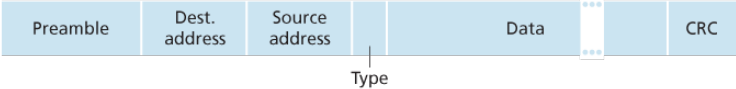
\includegraphics[width=\textwidth]{EthernetFrame.png}
\caption{Struttura di un frame ethernet}
\end{figure}
I campi di un frame ethernet sono:
\begin{itemize}
\item Data field (46 - 1500 bytes): trasporta il datagramma IP, ethernet ha una MTU (maximum transmission unit) di 1500 bytes. Se il datagramma supera questa dimensione deve essere frammentato e se ha
una dimensione minore di 46 bytes deve essere riempito per raggiungere quel valori.
\item Destination address (6 bytes): contiene l'indirizzo MAC dell'adattatore di destinazione che scarter\`a tutti i frame con un MAC diverso dal proprio.
\item Source address (6 bytes): contiene l'indirizzo MAC dell'origine del frame.
\item Type field (2 bytes): permette a ethernet di fare multiplex al protocollo del livello di rete (in modo da riconoscere quello utilizzato).
\item Cyclic redundancy check (4 bytes): utilizzato per controllare errori.
\item Preamble (8 bytes): i primi 7 bytes hanno un valore di $10101010$, l'ultimo di $10101011$. I primi byte servono a svegliare l'adattatore ricevente e per sincronizzare gli orologi. L'ultimo bit serve a 
segnalare la fine del preambolo.
\end{itemize}
Tutte le tecnologie ethernet mettono a disposizione un servizio senza connessione al livello di rete e non affidabile: non ci sono acknowledgments, un frame sbagliato viene eliminato. Utilizza il protocollo 
CSMA/CD.
\subsection{Switches di livello di link}
Il ruolo di uno switch \`e di ricevere frames e fare forwarding verso link in uscita. \`E trasparente agli host e ai router. Possiedono output buffer.
\subsubsection{Forwarding e filtering}
Filtering \`e la funzione che determina se un frame deve essere inoltrato a un'interfaccia o dovrebbe essere droppato. Forwarding \`e la funzione che determina l'interfaccia verso la quale un frame dovrebbe
essere diretto e lo muove in quella posizione. Entrambe le funzioni sono fatte attraverso una switch table che contiene entries per host e router nella LAN. Un entry contiene un indirizzo MAC, l'interfaccia dello
switch che conduce verso quell'indirizzo e il tempo in cui l'entry \`e stata messa nella tabella. Quando un frame entra in uno switch ci sono tre possibilit\`a:
\begin{itemize}
\item Se non c'\`e un entry per il MAC del destinatario lo invia a tutte le interfacce tranne quella di arrivo.
\item Se c'\`e un entry che associa il MAC con l'interfaccia di arrivo il pacco viene scartato. 
\item Se c'\`e un entry con interfaccia diversa viene inoltrato verso quell'interfaccia.
\end{itemize}
\subsubsection{Costruzione della tabella dello switch}
La tabella \`e costruita automaticamente, dinamicamente e autonomamente:
\begin{itemize}
\item La tabella \`e inizialmente vuota.
\item Per ogni frame in arrivo su un'interfaccia lo switch salva nella sua tabella l'indirizzo MAC, l'interfaccia da cui \`e arrivato e il tempo corrente in modo da avere la corrispondenza interfaccia-mittente.
\item Lo switch elimina un indirizzo se nessun frame \`e ricevuto con quell'indirizzo per un certo periodo di tempo. 
\end{itemize}
\subsubsection{Propriet\`a dello switching del livello di link}
\begin{itemize}
\item In una LAN costruita con switches non avvengono collisioni in quanto i  buffer frames non trasmettono mai pi\`u di un frame su un segmento.
\item Link eterogenei: essendo che uno switch isola un link dagli altri i link diversi in una LAN possono utilizzare tecnologie e velocit\`a diverse.
\item Aiutano la gestione bloccando link malfunzionanti e raccogliendo dati. 
\end{itemize}
\subsubsection{Router vs switch}
Gli switches sono plug-and-play, hanno tassi di flitering e forwarding alti, ma la topologia deve limitarsi ad uno spanning tree e sono suscettibili a broadcast storm. I router invece possono permettersi topologie
cicliche, mettono a disposizione protezione verso le broadcast storm, ma devono essere configurati e hanno un process time per pacchetto pi\`u elevato.
\subsection{Virtual Local Area Networks (VLANs)}
Una switched LAN organizzata gerarchicamente ha tre difetti:
\begin{itemize}
\item Mancanza di isolamento del traffico: i messaggi di broadcast vengono mandati a tutta la rete. 
\item Uso inefficiente degli switches. 
\item Gestire utenti: lo spostamento di utenti deve portare un utente a cambiare switch.
\end{itemize}
Queste difficolt\`a possono essere superate da uno switch che supporta una virtual local area network che permette multiple LAN virtuali di essere definiti lungo una singola fisica infrastruttura LAN.  Host in
una VLAN comunicano come se fossero connesso allo stesso switch. In una VLAN basata sulle porte le interfacce dello switch sono separate in gruppi che individuano le VLAN e formano un dominio di 
broadcasting. Per passare informazioni tra VLAN si dedica una porta ad un router e si dichiara quella porta come appartenente a tutte le VLAN dello switch. Un modo per scalare l'interconnessione di switches
VLAN \`e detto VLAN trunking in cui una porta speciale su ogni switch \`e configurata come una trunk port per interconnettere i due switches VLAN. La porta di trunk appartiene a tutte le VLAN e i frame inviati
in ogni VLAN sono forwarded lungo il trunk link. Per identificare l'appartenenza di un frame ad una particolare VLAN quando passa una trunk port viene esteso il protocollo ethernet con una VLAN tag di 
quattro byte che identifica la VLAN di appartenenza. 
\section{Virtualizzazione dei link: una rete come un link layer}
Reti Multiprotocol Label Switching (MPLS) sono reti packet-switched con circuiti virtuali. Ha il proprio formato di pacchetti e comportamenti di forwarding. Da un punto di vista dell'internet si possono
considerare come tecnologia di livello di link che server per interconnettere dispositivi IP. 
\subsection{Multiprotocol Label Switching}
MPLS hanno lo scopo di aumentare l'infrastruttura IP per etichettare selettivamente datagrammi e permettere ai router di fare forwarding basato su etichette di lunghezza fissa dove possibile. Un frame di 
livello di link gestito da un router capace di MPLS possiede un header MPLS tra l'header di livello link e rete. Tra i campi dell'header MPLS si trova l'etichetta, 3 bit per uso sperimentale, un bit singolo S utilizzato
per indicare la fine di MPLS header staccati e un campo time-to-live. Tale frame pu\`o essere inviato solo tra router capaci di MPLS denominati come label-switched router in quanto fanno forwarding attraverso
il lookup attraverso l'etichetta MPLS nella sua tabella di forwarding. Questo router pertanto non deve estrarre l'indirizzo IP di destinazione. MPLS permette di sovrascrivere routing IP e forzare del traffico lungo 
cammini diversi. Pu\`o essere utilizzato per rigenerare cammini di forwarding, facendo rerouting del traffico lungo in precomputato cammino in risposta al fallimento di link. Viene utilizzato nelle VPNs per isolare
le risorse e indirizzamento utilizzato dall'utente dagli altri. 
\section{Data center networking}
Ogni data center possiede la propria rete che interconnette i suoi host e interconnette il data center con l'internet. Gli host in un data server mettono a disposizione contenuti, salvano file e eseguono 
computazioni distribuite. Questi host sono chiamati blades e sono messi in rack al sopra del quale si trova un Top of Rack (TOR) switch che interconnette gli host nel rack tra di loro e con gli altri switches nel
data center: ogni host possiede un'interfaccia di rete che connette allo switch TOR e ogni switch TOR ha porte addizionali che possono essere connesse agli altri switches. Questo tipo di rete supporta due tipi
di traffico: quello tra host interni ed esterni e quello tra host interni. Per gestire il flusso con l'esterno si trovano dei border routers che connettono il data center all'internet. 
\subsection{Load balancing}
Un data center mette a disposizione molte applicazioni contemporaneamente e per gestire le richieste ogni applicazione possiede un indirizzo IP pubblico al quale clients inviano le loro richieste e dal quale 
ricevono risposte. All'interno del data center le richieste sono direzionate ad un load balancer il cui scopo \`e distribuire le richieste agli host in modo da equilibrare il carico tra gli host. Quando riceve una 
richiesta per un'applicazione particolare il load balancer la forward ad un host che gestisce l'applicazione. Quando l'host termina invia la risposta al load balancer che la ripassa al client esterno.  Oltre ad 
equilibrare la carica mette a disposizione una funzione simile al NAT traducendo l'indirizzo IP pubblico in quello interno.
\subsection{Struttura gerarchica}
Per scalare un data center di grande dimensioni viene utilizzata una gerarchia di router e switches. Alla cima della gerarchia il border router si connette all'access router, sotto di questi ci sono tre livelli di 
switches: ogni access router si connette ad uno switch top tier che si connettono a loro volta a multipli switches second tier e ad un load balancer. Ogni second tier switch si connette a multipli switch TOR. 
Quando il flusso di dati diventa importante si deve prestare attenzione a supportare comunicazione host-to-host con grande bandwidth. 
\section{Una Web Page request}
\subsection{DHCP, UDP, IP e ethernet}
Quando ci si connette ad una rete, prima di poter fare qualsiasi cosa si deve ottenere un indirizzo IP, il client pertanto deve eseguire il protocollo DHCP per ottenerlo.
\begin{itemize}
\item Il sistema operativo del client crea un DHCP request message in un segmento UDP con porta di destinazione 67 e di origine 68 che viene piazzato in un datagramma IP per il broadcast con indirizzo 
255.255.255.255 e uno di origine 0.0.0.0 in quanto non possiede ancora un indirizzo IP.
\item Il datagramma IP contenente il DHCP request message \`e piazzato in ethernet frame con un MAC FF:FF:FF:FF:FF:FF per il broadcast e il MAC di origine. 
\item Il frame \`e inviato allo switch che fa il broadcast verso tutte le porte di uscita. 
\item Il router riceve il broadcast ethernet frame ed estrae il datagramma IP il cui broadcast IP indica che dovrebbe essere processato dai protocolli di pi\`u alto livello in questo nodo, pertanto il segmento UDP
\`e demultiuplexes a UDP e il messaggio viene estratto dal segmento. Il server DHCP ha ora il DHCP request message.
\item Il server alloca un nuovo indirizzo IP e crea un DHCP ACK message che lo contiene con quello del server DNS, per il default gateway router e la network mask. Il messaggio viene messo in un segmento 
UDP, in un datagramma IP e in un frame ethernet. 
\item Questo frame viene inviato dal router allo switch che conosce l'indirizzo del destinatario indicato nel frame e lo invia al client.
\item Il client riceve il frame, estrae il datagramma, il segmento e il DHCP ACK message e il DHCP client registra l'indirizzo IP proprio, del server DNS del default gateway nella sua tabella di forwarding. 
\end{itemize}
\subsection{DNS e ARP}
Quando il client richiede una web page crea un socket TCP per inviare la richiesta HTTP. Per creare il socket il client deve conoscere l'indirizzo IP del destinatario.
\begin{itemize}
\item Il sistema operativo del client crea un DNS 	query message con il nome del destinatario che \`e piazzato in un segmento UDP con porta di destinazione 53, messo in un datagramma IP con indirizzo di 
destinazione del server DNS ritornato da DHCP. 
\item Il datagramma viene messo in un frame ethernet che viene inviato al gateway router di cui deve conoscere l'indirizzo MAC attraverso il protocollo ARP.
\item Il client crea un ARP query message con indirizzo IP del default gateway e lo piazza in un ethernet frame con una definizione di broadcast e lo invia nello switch che lo invia  a tutti i dispositivi connessi.
\item Il gateway router riceve il frame che contiene il messaggio ARP e prepara un ARP reply indicando il suo indirizzo MAC e lo piazza in un frame ethernet con indirizzo di destinazione del MAC del client.
\item Il client riceve il frame e estrae l'indirizzo MAC del gateway router.
\item Il client pu\`o ora indirizzare il frame ethernet contenente la query DNS verso il gateway router che riceve il frame contenente il datagramma IP con la DNS query.
\end{itemize}
\subsection{Intra-domain routing al server DNS}
\begin{itemize}
\item Il gateway router riceve il frame e estrae il datagramma IP contenente la DNS query. Fa un lookup per l'indirizzo di destinazione del datagamma e determina che la destinazione. Il datagramma viene 
messo in un frame e viene inviato lungo questo link.
\item Questo nuovo router riceve il frame, estrae il datagramma IP esamina l'indirizzo di destinazione e determina l'interfaccia di output verso il server DNS dalla tabella di forwarding riempita attraverso un
intra-domain protocol e BGP.
\item Alla fine il datagramma IP arriva al server DNS che estrae il DNS query message fa il lookup del nome  e trova il resource record che lo contiene e forma un DNS reply message che contiene la mappatura
hostname-to-IP, lo piazza in un segmento UDP e in datagramma IP e lo ritorna al client come nei passi precedenti.
\item Il client estrae l'indirizzo IP del server dal messaggio DNS ed \`e pronto a contattarlo.
\end{itemize}
\subsection{TCP e HTTP}
\begin{itemize}
\item Adesso che il client possiede l'indirizzo IP del server pu\`o creare il socket TCP che verr\`a utilizzato per mandare il messaggio HTTP GET. Quando il client crea il socket TCP viene eseguito il three-way
handshake con il TCP nel server. Pertanto crea un segmento TCP SYN con porta di destinazione 80 e lo mette in un datagramma IP con destinazione l'indirizzo IP del server, lo mette in un frame con indirizzo 
MAC del gateway router e lo invia allo switch.
\item I router nel cammino fanno forwarding verso il server utilizzando le loro tabelle di forwarding determinate dal protocollo DGP.
\item Il datagramma arriva al server che estrae il messaggio TCP SYN e fa demultiplexing verso il socket associato alla porta 80. Un socket di connessione \`e creato per la connessione tra il server HTTP e il 
client. Viene generato un segmento TCP SYNACK che \`e piazzato in un datagramma indirizzato al client e ad un frame appropriato.
\item Tale segmento viene inviato al client che fa demultiplexing verso il socket TCP creato precedente che entra nello stato di connessione.
\item Con il socket pronto per inviare bytes al server viene creato un messaggio HTTP GET che contiene l'URL che deve essere recuperato. Viene scritto nel socket e incapsulato in un segmento TCP.
\item Il server HTTP legge il messaggio HTTP GET e crea un messaggio di HTTP response in cui piazza il contenuto della web page richiesta nel corpo del messaggio e lo invia al socket TCP.
\item Il datagramma arriva al client e il programma legge l'HTTP response, estrae l'html dal corpo e mostra la web page. 
\end{itemize}